
%(BEGIN_QUESTION)
% Copyright 2009, Tony R. Kuphaldt, released under the Creative Commons Attribution License (v 1.0)
% This means you may do almost anything with this work of mine, so long as you give me proper credit

Write a PLC program that accepts two discrete input signals (from two switches), and outputs the following four discrete outputs:

\begin{itemize}
\item{} Output channel \#1: The status of input switch \#1 (simply repeating input \#1)
\vskip 5pt
\item{} Output channel \#2: The Boolean complement (opposite) of input switch \#1
\vskip 5pt
\item{} Output channel \#3: The {\tt AND} function of switches \#1 and \#2
\vskip 5pt
\item{} Output channel \#4: The {\tt OR} function of switches \#1 and \#2
\end{itemize}

\noindent
Shown here is a generic RLL listing of such a program:

$$\includegraphics[width=15.5cm]{i03667x01.eps}$$

\vskip 10pt

Turn on status highlighting within the programming software environment so that you may see the virtual ``power'' flow through the ``conductive'' contacts as you test the program.

\vskip 10pt

\vskip 20pt \vbox{\hrule \hbox{\strut \vrule{} {\bf Suggestions for Socratic discussion} \vrule} \hrule}

\begin{itemize}
\item{} How are discrete input and output points associated with contacts and coils in the ladder-logic program? 
\item{} How do you draw vertical connecting lines in the ladder-logic program? 
\item{} How do you assign ``alias'' names to inputs and outputs for easier program readability?  For example, how do you assign an English name to the input {\tt I:2/4} (Input channel 4 on card 2) on an Allen-Bradley SLC 500 PLC so that it reads as ``Input\_switch\_4'' in the program instead of ``{\tt I:2/4}'' in the programming software's display?
\item{} Where is the software function (pull-down menu option, button, hot-key, etc.) located that allows you to turn on contact status highlighting in the PLC programming software?
\end{itemize}

%\vskip 10pt

%\noindent
%PLC comparison:

%\medskip
%\item{} \underbar{Allen-Bradley Logix 5000}: 
%\vskip 5pt
%\item{} \underbar{Allen-Bradley SLC 500}: 
%\vskip 5pt
%\item{} \underbar{Siemens S7-200}:
%\vskip 5pt
%\item{} \underbar{Koyo (Automation Direct) DirectLogic}:
%\medskip

\underbar{file i03667}
%(END_QUESTION)





%(BEGIN_ANSWER)

 
%(END_ANSWER)





%(BEGIN_NOTES)

I strongly recommend students save all their ``exploratory'' PLC programs for future reference, commenting them liberally and saving them with special filenames for easy searching at a later date!

\vskip 10pt

I also recommend presenting these ``exploratory'' programs as problems for students to work on in class for a short time period, then soliciting screenshot submissions from students (on flash drive, email, or some other electronic file transfer method) when that short time is up.  The purpose of this is to get students involved in PLC programming, and also to have them see other students' solutions to the same problem.  These screenshots may be emailed back to students at the conclusion of the day so they have other students' efforts to reference for further study.

%INDEX% PLC, exploratory question (ladder logic programming)

%(END_NOTES)


